\section{TCN}
\begin{frame}[c]{An Empirical Evaluation of Generic Convolutional and Recurrent Networks for Sequence Modeling}
\begin{itemize}
	\setbeamertemplate{itemize items}[square]
	\item Утверждается, что сверточные нейронные сети подходят для задач NLP лучше RNN.
	\item Предлагаются методы обучения глубоких временных сверточных сетей (TCN).
\end{itemize}
\let\thefootnote\footnote{\href{http://arxiv.org/abs/1803.01271}{\color[rgb]{0.5,0.5,0.5} [Bai et al., 2018]}}
\end{frame}

\begin{frame}[c]{An Empirical Evaluation of Generic Convolutional and Recurrent Networks for Sequence Modeling}
\begin{figure}
	\centering
	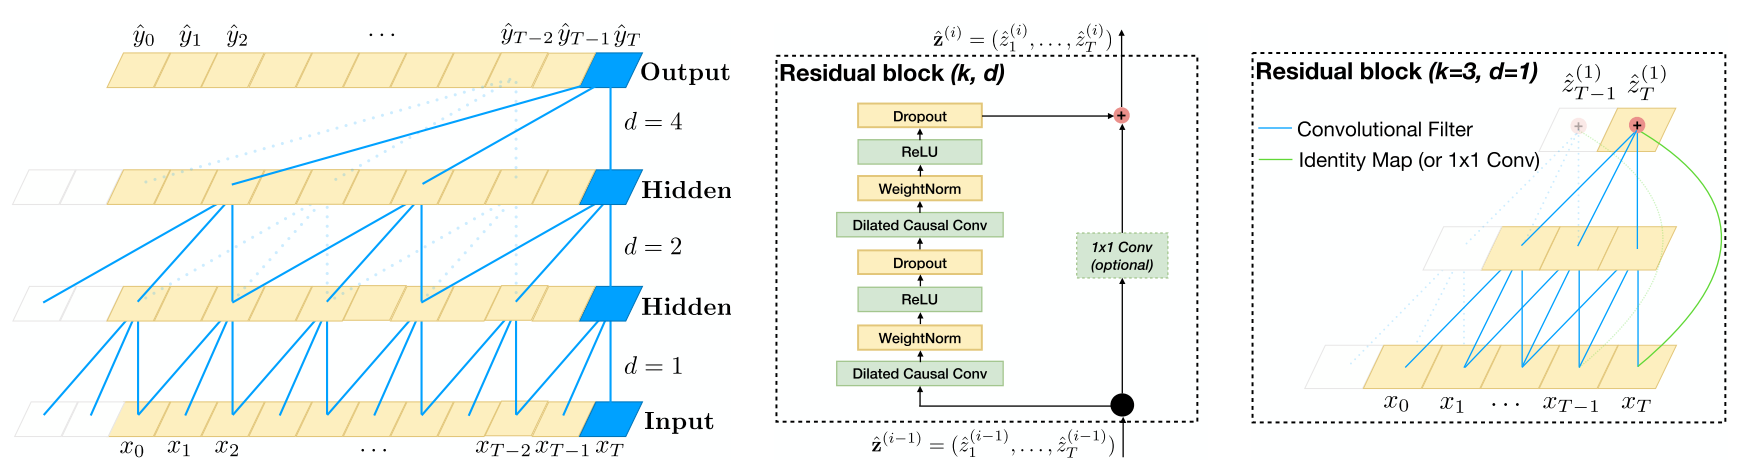
\includegraphics[width=1.0\textwidth]{figures/tcn.png}
\end{figure}
\begin{itemize}
	\setbeamertemplate{itemize items}[square]
	\item Causal convolutions: выход в момент времени $t$ зависит только от элементов из времени $t$ и ранее в предыдущем слое.
	\item Dilated Convolutions: экспоненциальный receptive field по глубине сети. 
	\item Residual Connections: способ проброса градиентов в глубину, не проходя через нелинейные функции активации.
\end{itemize}
\end{frame}

\begin{frame}[c]{An Empirical Evaluation of Generic Convolutional and Recurrent Networks for Sequence Modeling}
\begin{itemize}
	\setbeamertemplate{itemize items}[square]
	\item В итоге:
	\begin{itemize}
		\setbeamertemplate{itemize items}[circle]
		\item Параллелизм. 
		\item Гибкий размер receptive field.
		\item Стабильные градиенты.
		\item Входы переменной длины.
	\end{itemize}
\end{itemize}
\end{frame}

\begin{frame}[c]{An Empirical Evaluation of Generic Convolutional and Recurrent Networks for Sequence Modeling}
\begin{itemize}
	\setbeamertemplate{itemize items}[square]
	\item Результаты на задаче языкового моделирования:
\end{itemize}
\begin{figure}
	\centering
	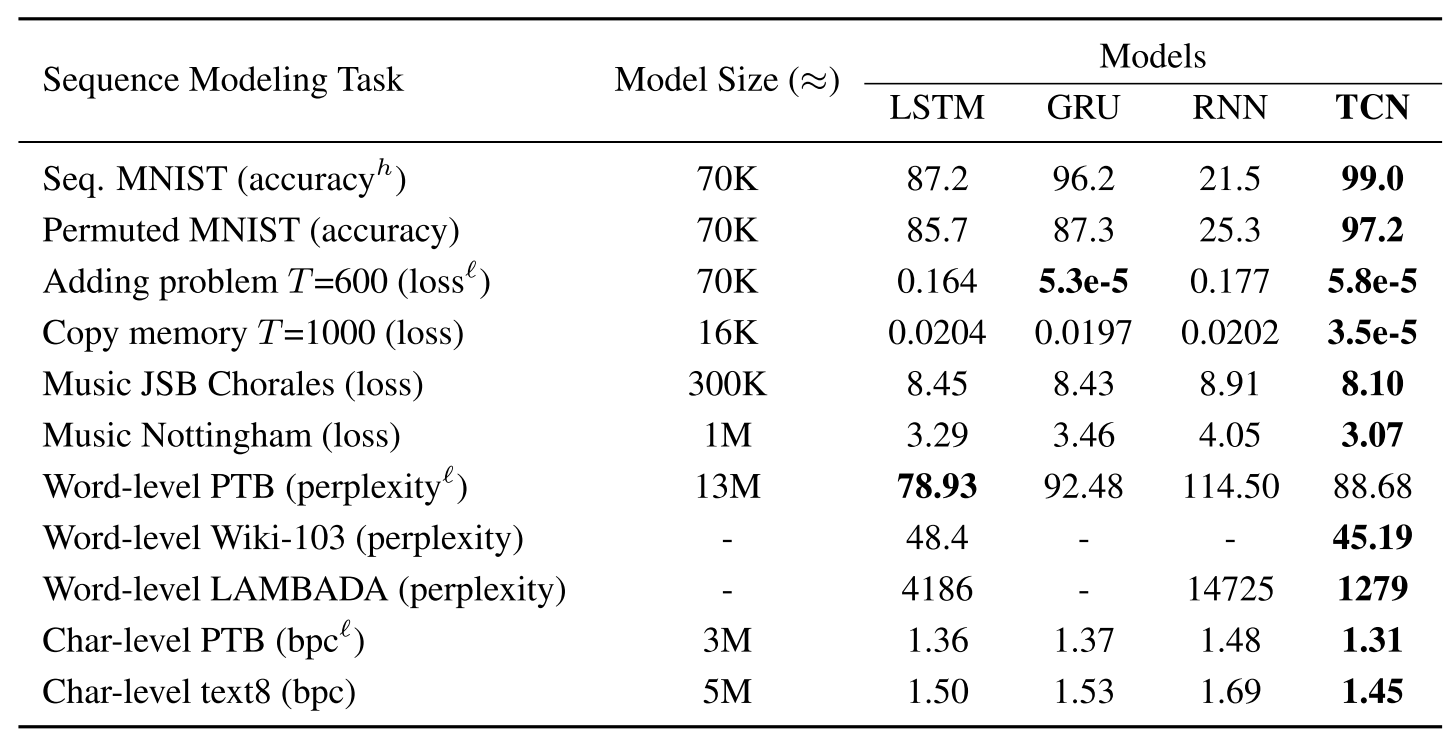
\includegraphics[width=1.0\textwidth]{figures/tcnres.png}
\end{figure}
\end{frame}